Please describe the basic characteristics of the software. 

Is is a web-based solution?

Ja

Is it installable or just available as a service? 

Die Software ist installierbar.



How much effort does the installation take (describe and give a time for the installation)?

Die folgenden Schritte werden auf folgendem Testrechner ausgef�hrt:

Ubuntu 12.04

Es wird die Free Trial Version von Nagios XI heruntergeladen unter:

http://www.nagios.com/products/nagiosxi

Die Trial Version ist eine 60 Tage Testversion von Nagios XI.

Es wird die VMware Virtual Machine (64-bit) Version 2012R1.6 heruntergeladen unter:

http://library.nagios.com/library/products/nagiosxi/downloads/main

Auf der viruellen Maschine l�uft CentOS 6.x und Nagios XI 2012 ist installiert.

Um die VMware Virtual Machine starten zu k�nnen, muss VMware installiert werden.
VMware kann kostenfrei heruntergeladen werden unter:

\url{https://my.vmware.com/web/vmware/free#desktop_end_user_computing/vmware_player/5_0}

Der heruntergeladene VMware-Player wird installiert mit:

sudo sh VMware-Player-5.0.1-894247.x86\_64.bundle

Der VMware-Player wird gestartet und es wird die virtuelle Maschine ausgew�hlt mit 

Open a virtual Maschine.

Die ausgew�hlte virtuelle Maschine wird gestartet mit 

play virtual maschine.

Die virtuelle Maschine wird gestartet. CentOS wird gebootet und Nagios gestartet.

Auf Nagios XI kann jetzt im Browser zugegriffen werde unter:

http://192.168.0.100/

\begin{figure}[htp]
\centering
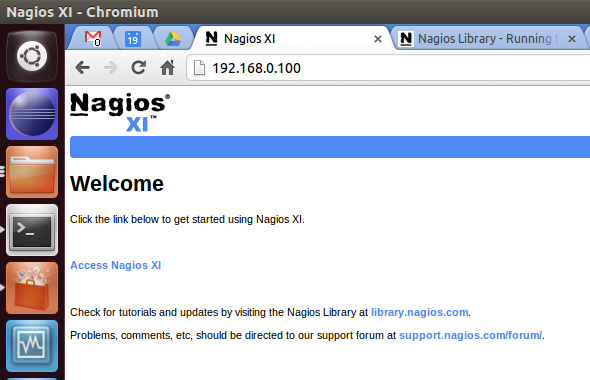
\includegraphics[width=0.6\textwidth]{ingo/bilder/Startseite}
\caption{Startseite von Nagios}
\label{fig:StartseiteVonNagios}
\end{figure}

Das Default Root Passwort ist nagiosxi


How old is the software? When did its development start? 

1999 ver�ffentlichte Ethan Galstad Nagios - dass damals noch NetSaint hie� - als Open Source Projekt.
http://www.nagios.org/about/history

Which version is it (0.1?)? 

Netsaint 0.0.1
\url{http://www.ussrback.com/UNIX/audit/netsaint/index.html}

Is it well established? How many customers are using it? 

Es wird gesch�tzt, dass es weltweit ca 1 Million Nagios Nutzer gibt.
http://www.nagios.org/about/community

Is it still further developed - are new releases planned and when was the last release?

Es wird immernoch weiterentwickelt. Neue Releases sind geplant. Die letzte Version 2012R1.6 ist von 15. Februar 2013.